\textbf{config: multiply implementation: 3 16-bit multipliers
        multiply extended implementation: 1 16}
        optimization level = O2, debug level = on
        \\
\textbf{Case1: }
config: multiply implementation: 3 16-bit multipliers
        multiply extended implementation: 1 16,
        optimization level = O2,
        \textbf{cosf}
Vector length (N)     = 52
Total ticks           = 105
Average ticks         = 5
Result f(x)           = 170105728.000000
Program size: 73 KBytes program size (code + initialized data).
              304 KBytes free for stack + heap.
\\
config: multiply implementation: 3 16-bit multipliers
        multiply extended implementation: 1 16,
        optimization level = O2
        \textbf{cos}
Vector length (N)     = 52
Total ticks           = 159
Average ticks         = 7
Result f(x)           = 170105728.000000
Program size: 74 KBytes program size (code + initialized data).
              302 KBytes free for stack + heap.
\\ 
mulhardware support + optimization level off, cosf
Vector length (N)     = 52
Total ticks           = 106
Average ticks         = 5
Result f(x)           = 170105728.000000
Program size: 76 KBytes program size (code + initialized data).
              301 KBytes free for stack + heap.
\\
mulhardware support + optimization level = O1, cosf
Vector length (N)     = 52
Total ticks           = 104
Average ticks         = 5
Result f(x)           = 170105728.000000
Program size: 73 KBytes program size (code + initialized data).
              303 KBytes free for stack + heap.
\\
mulhardware support + optimization level = O3, cosf
Vector length (N)     = 52
Total ticks           = 105
Average ticks         = 5
Result f(x)           = 170105728.000000
Program size: 73 KBytes program size (code + initialized data).
              304 KBytes free for stack + heap.
\\
mulhardware support + optimization level = size, cosf
Vector length (N)     = 52
Total ticks           = 104
Average ticks         = 5
Result f(x)           = 170105728.000000
Program size: 73 KBytes program size (code + initialized data).
              304 KBytes free for stack + heap.



Case2: 
\textbf{COSF}
Vector length (N)     = 2041
Total ticks           = 4090
Average ticks         = 204
Result f(x)           = 6627435008.000000
Program size: 81 KBytes program size (code + initialized data).
              296 KBytes free for stack + heap.
\textbf{COS}
Vector length (N)     = 2041
Total ticks           = 6199
Average ticks         = 309
Result f(x)           = 6627435520.000000
Program size: 82 KBytes program size (code + initialized data).
              295 KBytes free for stack + heap.
\\
mulhardware support + optimization level = off, cosf
Vector length (N)     = 2041
Total ticks           = 4133
Average ticks         = 206
Result f(x)           = 6627435008.000000
Program size: 84 KBytes program size (code + initialized data).
              293 KBytes free for stack + heap.
\\
mulhardware support + optimization level = O1, cosf
Vector length (N)     = 2041
Total ticks           = 4041
Average ticks         = 202
Result f(x)           = 6627435008.000000
Program size: 81 KBytes program size (code + initialized data).
              296 KBytes free for stack + heap.
\\
mulhardware support + optimization level = O3, cosf
Vector length (N)     = 2041
Total ticks           = 4090
Average ticks         = 204
Result f(x)           = 6627435008.000000
Program size: 81 KBytes program size (code + initialized data).
              296 KBytes free for stack + heap.


Case3:
\textbf{COSF}
Vector length (N)     = 65281
Total ticks           = 131279
Average ticks         = 6563
Result f(x)           = 211932430336.000000
Program size: 328 KBytes program size (code + initialized data).
              49 KBytes free for stack + heap.
\textbf{COS}
Vector length (N)     = 65281
Total ticks           = 198847
Average ticks         = 9942
Result f(x)           = 211932413952.000000
Program size: 329 KBytes program size (code + initialized data).
              48 KBytes free for stack + heap.
\\
mulhardware support + optimization level = off, cosf
Vector length (N)     = 65281
Total ticks           = 132405
Average ticks         = 6620
Result f(x)           = 211932430336.000000
Program size: 331 KBytes program size (code + initialized data).
              46 KBytes free for stack + heap.
\\
mulhardware support + optimization level = O1, cosf
Vector length (N)     = 65281
Total ticks           = 129542
Average ticks         = 6477
Result f(x)           = 211932430336.000000
Program size: 328 KBytes program size (code + initialized data).
              49 KBytes free for stack + heap.
\\
mulhardware support + optimization level = O3, cosf
Vector length (N)     = 65281
Total ticks           = 131312
Average ticks         = 6565
Result f(x)           = 211932430336.000000
Program size: 328 KBytes program size (code + initialized data).
              49 KBytes free for stack + heap.
\\
mulhardware support + optimization level = size, cosf
Vector length (N)     = 65281
Total ticks           = 129047
Average ticks         = 6452
Result f(x)           = 211932430336.000000
Program size: 328 KBytes program size (code + initialized data).
              49 KBytes free for stack + heap.



Case4:
\textbf{COSF}
Vector length (N)     = 2323
Total ticks           = 4645
Average ticks         = 232
Result f(x)           = 7668609536.000000
Program size: 82 KBytes program size (code + initialized data).
              295 KBytes free for stack + heap.

\textbf{COS}
Vector length (N)     = 2323
Total ticks           = 7124
Average ticks         = 356
Result f(x)           = 7668609024.000000
Program size: 83 KBytes program size (code + initialized data).
              294 KBytes free for stack + heap.
\\
mulhardware support + optimization level = off, cosf
Vector length (N)     = 2323
Total ticks           = 4742
Average ticks         = 237
Result f(x)           = 7668609536.000000
Program size: 85 KBytes program size (code + initialized data).
              292 KBytes free for stack + heap.
\\
mulhardware support + optimization level = O1, cosf
Vector length (N)     = 2323
Total ticks           = 4712
Average ticks         = 235
Result f(x)           = 7668609536.000000
Program size: 82 KBytes program size (code + initialized data).
              294 KBytes free for stack + heap.
\\
mulhardware support + optimization level = O3, cosf
Vector length (N)     = 2323
Total ticks           = 4647
Average ticks         = 232
Result f(x)           = 7668609536.000000
Program size: 82 KBytes program size (code + initialized data).
              295 KBytes free for stack + heap.
\\
mulhardware support + optimization level = size, cosf
Vector length (N)     = 2323
Total ticks           = 4694
Average ticks         = 234
Result f(x)           = 7668609536.000000
Program size: 82 KBytes program size (code + initialized data).
              295 KBytes free for stack + heap.



\begin{figure}[H]
    \centering
    \fbox{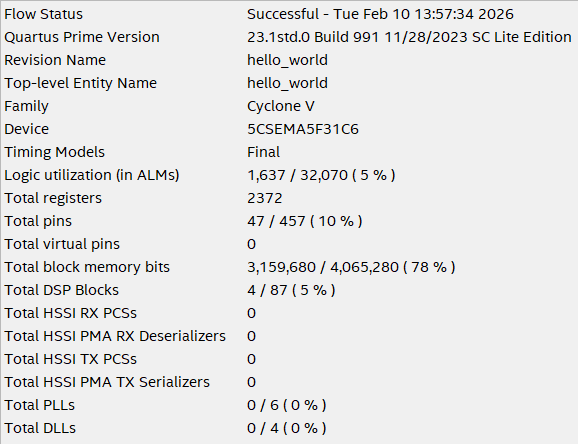
\includegraphics[width=0.95\linewidth]{Images/task4-1.png}}
    \caption{Task 3 FPGA resource utilization snapshot.}
    \label{fig:task4_resource_placeholder}
\end{figure}

